% 
%% SOSP 2017 Template
%%
%% Uses sigplanconf from:
%% 
%%    http://www.sigplan.org/sites/default/files/sigplanconf.cls
%%
%% with 10pt and preprint options. 
%%
%% Replace 'XX' with your paper number (assigned when you register abstract)
%% Replace 'NN' with actual number of pages. 

\documentclass[10pt,preprint,nocopyrightspace]{sigplanconf}
\usepackage{times}

\usepackage{datetime}
\usepackage{url}
\usepackage{hyperref}
\usepackage{graphicx}
\usepackage{grffile}
\usepackage[T1]{fontenc}
\usepackage{listings}
\usepackage{float}
\usepackage{natbib}

\bibliographystyle{IEEEtran}
\setcitestyle{numbers,square,comma, sort&compress}


% These only appear when the 'preprint' option is specified.
% Enabling these will cause the first page of the document to fail the 
% format check on HotCRP :-(
%\titlebanner{Under submission to SOSP 2017 - do not cite or distribute}
%\preprintfooter{Draft of {\currenttime}, \today{}}

% No date in title area.
\date{}

% Paper number and no. of pages as author
\authorinfo{\textbf{\#01}}{6 pages - draft}


% Actual document begins below.
\begin{document}

\title{f9: A secure microkernel for MMUless embedded systems} 
\maketitle

\begin{abstract}\textsl{}
	
Internet of Things (IoT) can be see in such as vehicle, sensors nodes, smartphones, and medical applicances today. The hardware of IoT are constrained in terms of computing power, avaliable memory, communication, and energy capacities, and the system of IoT is expected to fulfill these requirements: reliability, real-time behavior. 

The concept of microkernel can fulfill the requirements of IoT devices, but microkernel approaches such as seL4, OKL4, still need a rich hardware resource with MMU for memory management and higher power consumption.

In this paper, we describe the design and implementation of f9-kernel - a microkernel based on L4 kernel family, aim to built for deeply embedded IoT devices for efficiency, security, and flexible development. F9 microkernel is optimized for ARM Cortex-M series CPU, with only 3500 lines of source code, which is the smallest microkernel in today.

\end{abstract}

\section{Introduction}

An OS for IoT devices should at lease fulfill the reliability\cite{baccelli2013riot}. Research in operating systems shows that monolithic kernel such as Linux kernel\cite{chou2001empirical} and Microsoft Windows NT\cite{swift2005improving} are making errors from drivers, and Heiser state that larger trusted computing base (TCB) cannot be made trustworthy, the key to a trustworthy TCB is a very small kernel\cite{heiser2005secure}, thus we are aim to use microkernel to fulfill reliability.

In microkernel, kernel only provides three mechanisms: IPC, Memory Management and thread management, and these mechanisms can be used to build up the services, for example file systems or device drivers, which can provide complete functions for unprivileged applications. 

The history of microkernel can be date back to 1969s, and have developed in 3 generations: (i) Mach, (ii) L3 \& L4, improving IPC performance, written in assembly (iii) seL4, Fiasco.OC, NOVA, platform independence and formal verification, security, SMP, etc. 



\section{Background of L4 microkernel}

Microkernel is a concept to build an minimality kernel, and f9-kernel is based on the L4 kernel, the basic mechanisms can be devided into three parts: inter-process communication (IPC), thread management, and low-level address space management.

\begin{figure}[H]
	\begin{center}
		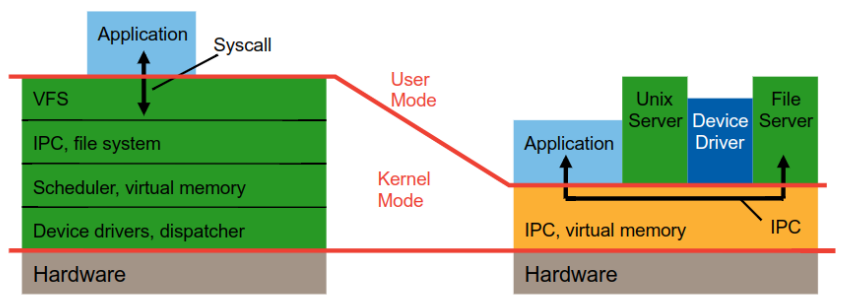
\includegraphics[width=\linewidth]{picture/kernel_diff.png}
	\end{center}
	\caption{kernel space service is split out to user space in microkernel \cite{heiser2012}}
	\label{fig:kernel_diff}
\end{figure}


\subsection{Inter-Process Communication}

Inter-Process Communication (IPC) is the mechanism that microkernel thread communicate with other threads\cite{liedtke1993improving}. IPC is an critical issue in microkernel since user code obtains a system service via IPC, typically message passing. IPC may design in synchronous or asynchronous, but in the principle of minimality, a kernel will only choose one approach. L4 kernel provides message-baced, synchronous IPC between threads for performance reason since liedtke reserach in 1993\cite{liedtke1993improving}, only OKL4 used the asynchronous IPC approach\cite{elphinstone2013l3}.

\subsection{Thread Managemnet}

Threads is the basic execution unit in L4. They are created, destroyed via the \verb|Thread-Control| system call\cite{nourai2005aphysically}. The thread dispatcher is responsible for switching contexts. Each thread has its own Thread Control Block (TCB) and addressed by its global id, the TCB is where a thread's state is saved to or restored from on a context switch\cite{nourai2005aphysically}.

\subsection{Thread identifiers}

Every threads in L4 have \textit{global} and \textit{local} thread identifier (thread id). Global thread id is unique throughout the entire system, local thread id have the scope limited in its own address space.

The global thread identifier in L4 contains two distinct parts - a upper 18-bits thread number and lower 14-bits version number. Also there are two special thread ids reserved L4 API - NilThread and AnyThread. NilThread identifier is implemented as 0, and AnyThread is impledmented as all bits set to 1. These special thread identifier will be used in L4 IPC system call\cite{nourai2005aphysically}.

\subsection{Memory Mnagement and Address spacecs }

In modern system architectures and operating system, physical memory usually will be 'virtualize' into virtual memory for programs to execute in\cite{arpaci2015operating}. A hardware device called memory-management unit (MMU) will translate between physical memory address to virtual memory and so on are lies between CPU and memory.

L4 provides the mechanism for implementing recursively-defined virtual address that are managed in user level\cite{dannowski2011l4}. Initial address space is controlled by first process, other process who derive from the first process, will obtain memory pages from first.

\section{Design of f9 kernel}

The f9 kernel is aim to run on the deep embedded devices, thus its goals is to make f9 kernel be efficiency and security.

\begin{figure}[H]
	\begin{center}
		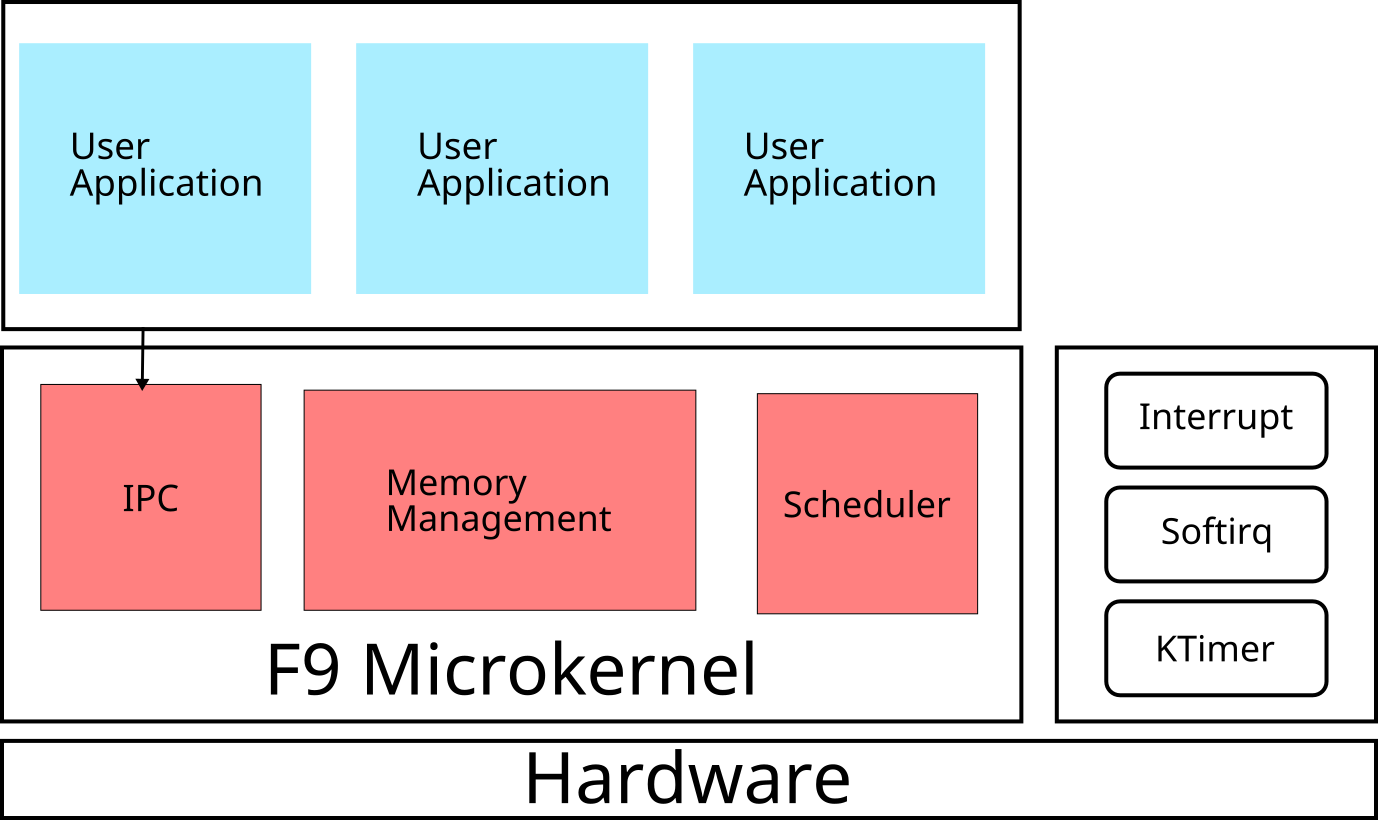
\includegraphics[width=\linewidth]{picture/f9_arch.png}
	\end{center}
	\caption{f9-kernel system architecture}
	\label{fig:f9}
\end{figure}

\subsection{Memory Management}

Unlike other L4 kernels, f9-kernel focus on MPU-only platform such as ARM cortex-M CPU, so we cannot use virtual memory for memory managements. Also, the RAM was small (256 Kbytes) but a larger Physical address space (up to 32-bit) was used, including the hardware device, flash, and bit-band zone, and only have 8 memory protection unit (MPU)\cite{arm2016mpu,yiu2013definitive,st2016managing,usna2015l18}.

MPU is a hardware unit that can set access control permissions for a memory region. There are 8 MPU in Cortex-M CPU, each of the MPU can set individual access permission for a memory region. There is a limitation of setting memory region in MPU is that developer can only set "$2^n$" size memory region from 32 bytes to 4 Gbytes\cite{yiu2013definitive,st2016managing}. For example, setting 64 bytes memory region is valid, but setting 96 bytes memory region is invalid. Obey to this limitation, f9-kernel developed an elegant mechanism to breakthrough this limited for memory management, called fpage.

Memory management in f9-kernel, can split into three conceptions: 1. memory pool, which represents the area of PAS with specific attributes (hardcoded in mem map table). 2. flexible page - unlike traditional pages in L4, fpage represent in MPU region instead. 3. address space - linked list of fpages bound to particular thread(s).

\subsubsection{Memory Pool}
In f9-kernel, memory pool was static and declare before compile; it will declare each memory segment's start, end, permission, etc., then slice the needed part into fpage size, put into address space.

\subsubsection{Address Space}
Address space is the structure that each thread record their fpage. When creating a new thread in f9-kernel, it will first declare fpage chain for it, then mapping needed information into address space.

Using \texttt{map{\_}area} function, \texttt{map{\_}area} can find the proper address space from source to destination by giving base position and size, it will search the first and last fpage that contain base position and end of the request size. If the first and last fpage was found, it will split fpage into two fpage, then mapping fpage from source to destination. f9-kernel provide these API for setting up address space: 
\begin{itemize}
\item \verb|as_create|
\item \verb|as_setup_mpu|
\end{itemize}

\verb|as_create| is used when creating a new thread, it will allocate an new address space from address space table.

\verb|as_setup_mpu| is used when perform context switch between two thread.


\subsubsection{Flexible pages (fpage)}
In f9-kernel, every fpage can directly use by MPU as a page (that mean be protected by MPU), and address space was build from fpage. Fpage structure include base address, memory pool id, flags, size and permission. f9-kernel provide fpage API:
\begin{itemize}
	\item \verb|create_fpage|
	\item \verb|create_fpage_chain|
	\item \verb|assign_fpages|
\end{itemize}

\subsection{IPC}

f9-kernel implemented very small set of system call from L4, one of the system call is IPC\cite{dannowski2011l4, arm2016svc}. f9-kernel IPC was implemented in synchronous IPC, means that when a thread want to communicate with another thread, it will first set sender into the \verb|SEND_BLOCKED| state, then waiting for target receiver goes into the \verb|RECV_BLOCKED| state. After these two threads are in the proper state, it will thus perform IPC communication. This technique avoids buffering in the kernel (cause no need for maintaining a buffer or queue for recv / send), the management and the copying cost between two thread.\cite{nourai2005aphysically}

f9-kernel introduce two different IPC register - message register and buffer register. The message register is a virtual register that can only be read one time, after one read, the value in this message register will be undefined. First introduced the concept in pistachio\cite{nourai2005aphysically}, Message register can be moderate-size and now f9-kernel implement 4 type of items: Untyped, Typed, Map, Grant item.

\subsection{IPC practial view}

IPC syscall in f9-kernel has send and receive two stage. If target thread wasn't waiting for receive, then caller thread will go into send block state until target thread starts to receiving.

And, receiving thread can set into two receive type: 1. closed receive: wait for particular thread. 2. open wait: wait for all thread who prepare to send to it.

We can study IPC from the classic program in l4 / 49 calls "Ping Pong," this program setting up two thread call "Ping" and "Pong," Ping will try to send a message to Pong by using IPC. Below is the pseudo code for ping and pong.

\begin{lstlisting}[language=c,frame=single,basicstyle=\small]
/* Ping */
L4_Msg_t msg;
L4_MsgTag_t tag;

L4_MsgClear(&msg);
L4_MsgLoad(&msg);

loop {
    tag = L4_Send(threads[PONG_THREAD]);
}

/* Pong */
L4_MsgTag_t tag;
L4_Msg_t msg;

loop {
    tag = L4_Receive(threads[PING_THREAD]);
    L4_MsgStore(tag, &msg);
}
\end{lstlisting}

We can see that Pong is using close receive to specify receive message from Ping thread, then Ping thread will send the message to Ping thread by calling \texttt{L4\_Send} function.

If we trace down the code, we can see that \texttt{L4\_Send} and \texttt{L4\_Recive} is only a convenience programming interface for \texttt{L4\_IPC} [7].

\begin{lstlisting}[language=c,basicstyle=\small,frame=single]
/* include/l4/ipc.h */
L4_MsgTag_t L4_Send(L4_ThreadId_t to)
{
    return L4_Ipc (to,
                   L4_nilthread,
                   L4_Never, 0);
}

/* user/lib/l4/platform/syscalls.c */
L4_MsgTag_t L4_Ipc(L4_ThreadId_t to,
           L4_ThreadId_t FromSpecifier,
           L4_Word_t Timeouts,
           L4_ThreadId_t *from)
{
    L4_MsgTag_t result;
    L4_ThreadId_t from_ret;

    __asm__ __volatile__(
        "svc %[syscall_num]\n"
        "str r0, %[from]\n"
        : [from] "=m"(from_ret)
        : [syscall_num] "i"(SYS_IPC));

        result.raw = __L4_MR0;

    if (from != NULL)
        *from = from_ret;

    return result;
}
\end{lstlisting}

The reason that we separate \texttt{L4\_IPC} and \texttt{L4\_Send} is because system call part is platform specific land, for the cross-platform issue, we put this code in a separate file. We can see \texttt{L4\_IPC} calling svc with \texttt{syscall\_num}; svc is the supervisor call in Cortex-M, witch request privileged operations or access to system resources from an operating system[8]. For calling convention, R0-R2 were saving to, FromSpecifier, and Timeouts, so from the receiver Pong \texttt{L4\_Receive}, it will take R0 as \texttt{L4\_nilthread}, R1 as Ping Thread and R2 as \texttt{L4\_Never}.
		
Then seek into the kernel, we can found that this is an \texttt{SYS\_IPC} call in kernel/ipc.c; then it will perform the proper IPC process. Because to thr is \texttt{L4\_nilthread}, so that we can know this \texttt{SYS\_IPC} call is a receive calling, and FromSpecifier wasn't ANYTHREAD, so this is a close receive specify for Ping Thread.
	
But if receiver and sender were not synchronous? They will only lock themselves and wait for \texttt{ipc\_deliver} to perform IPC communicate. \texttt{ipc\_deliver} is a function that ticks from kernel timer every 64 ticks to do with two IPC communicate.

\begin{lstlisting}[basicstyle=\small,frame=single]
/* psudocode for ipc_deliver event */
ktimer_event_create(64, ipc_deliver, 0);
\end{lstlisting}

\subsection{scheduler}

The thread scheduler in f9-kernel have the responsibility to select new thread for context switches, it perfrom as a round-robin scheduler, and tries to select the first runnable normal thread. In f9-kernel, all threads are at the same priority, this causes the problem if user space thread was a busy loop, it will hang on busy loop thread and never transfer to other normal thread.

\begin{figure}[H]
	\begin{center}
		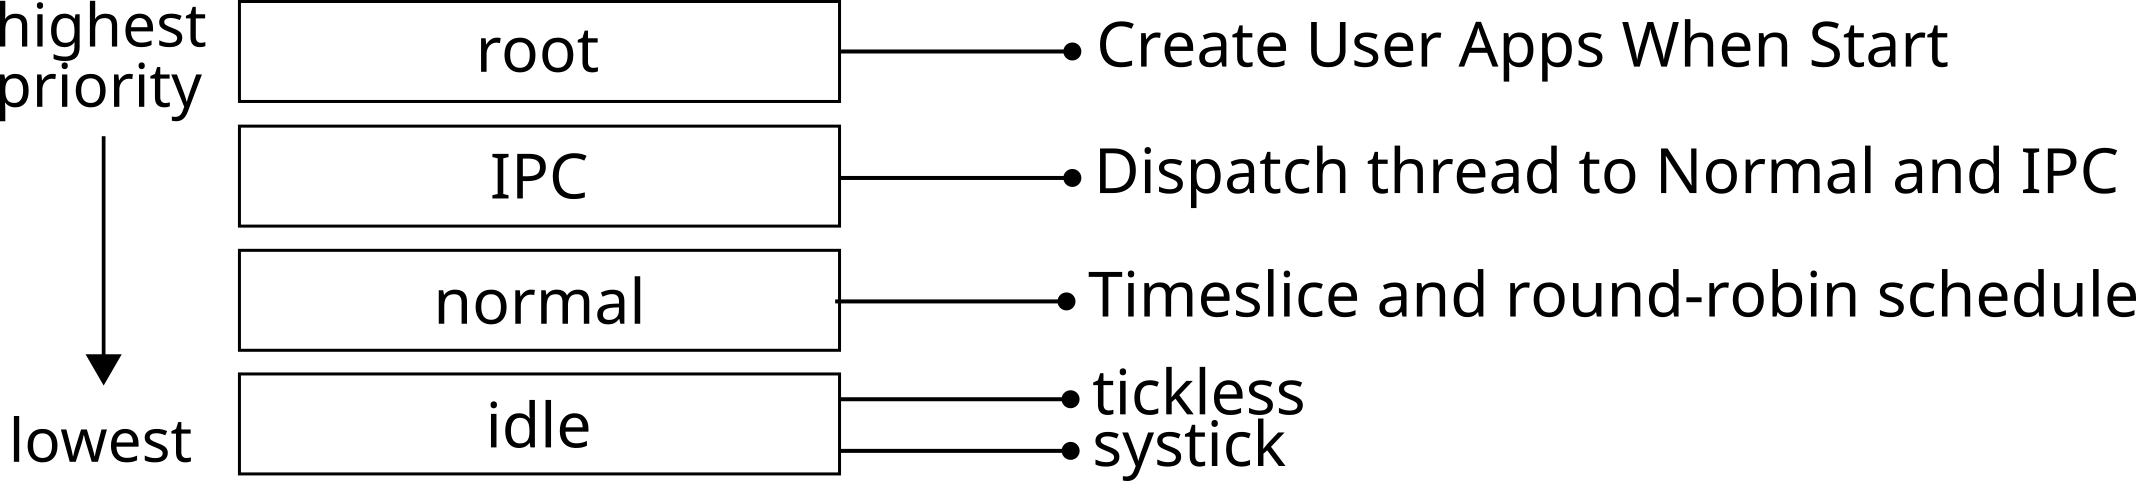
\includegraphics[width=\linewidth]{picture/scheduler.png}
	\end{center}
	\caption{f9-kernel scheduler hierarchy}
\end{figure}

So now we are trying to create a pluggable scheduler framework on f9-kernel.  Fi-asco.OC has similar approach\cite{elphinstone2013l3,fiasco}.

\section{Implementation techniques}

實際上有很多限制,in deterministic, microscope 最佳化, 又要系統很好維護
robert love, 

\subsection{sorting}
f9-kernel sort routines is token from BSD\cite{bentley1993engineering}, BSD approach found that swapping is the most sensitive issue in sorting. It have conqure the problem that sorting in differnet width data size. Also f9-kernel implement sort by heapsort to prevent quick sort worst case in $\mathcal{O}(n \times n)$ , make the sorting time is $\mathcal{O}(n\log{}n)$  both on average and worst-case.

\subsection{memcpy, duff's device}
f9-kernel memcpy was derive from MUSL libc project\cite{felker}, it using the technique from "Duff's device", also called "loop unrolling" to improve the performance of memcpy. The future work is to rewrite memcpy code in ARM Thumb-2 to improve performance.

\subsection{Init hooks}

f9-kernel used an techqunie call "Initialize hooks", this technique can let developer write code in kernel and assign to run the code in specific stage when kernel is initializing.

f9-kernel provide an API \verb|INIT_HOOK(hook, level)|, this is a syntactic sugar that will convert into an const \verb|init_struct|, which will then put in section \verb|.init_hook|, in linker script it will define \verb|init_hook| start and end position, it will be an linear address for all init hook define by developer.

In booting stage, kernel will try to execute these hook by \verb|run_init_hook(level)|, this function will then scan the \verb|init_hook| region from start to end, if it found the proper level to execute, it will then execute the hook. Also, when multiple hooks are in the same level, this approach won't guarantee the order to execute hooks.

\subsection{Ksymbol maps and Kprobe}
f9-kernel using an elegant method to dump out symbol from kernel and let kernel can using these symbol information such as function address and symbol name in runtime. When building the entire kernel, build system will first compile all component then linked to a non-symbol elf kernel file, then the special make scripts which build for covert elf to symbol map file, will using GNU toolchain "nm" tool to dump all symbols out of the kernel into a pre-define c template. After all, it compile and linked the non-symbol kernel and symbol map which set into the \texttt{.sym\_tab} section.

This mechanism let f9-kernel can easily using symbol maps in runtime, and the demostration about using sybmol map can be found at Kprobe.

f9-kernel have implement an light weight debugging system call "Kprobe", this term is inherit from Linux kernel. The Kprobe goals is to provide an in-kernel dynamic tracing mechanism, allow developers to gather additional infromation about kernel operation without recompiling or rebooting system. Currently, Kprobe is implemented through hardware breakpoint from ARMv7 Debug Architecture. 

In ARMv7, we can use DebugMon exception to trap probed address\cite{yiu2013definitive}, when a kprobe is registered, one of the FPB (Flash patch and Breakpoint Unit) will set to the probed address. When a CPU hits the probed address, trap occurs, FPB will generate a DebugMon exception and set bit-BKPT in Debug Fault Status Register (DFSR).

After all \texttt{pre\_handlers} of kprobes associated with the probed address arecalled, Kprobes sets \texttt{bit-MON\_STEP} in Debug Exception and Monitor Control Register in order to single-step the probed address; Then Kprobes returns to
the probed address. And soon a DebugMon exception will be generated againonce an instruction is executed.

We can check bit-HALTED from DFSR to know if there is a single-step debug event. If yes, it is time to call all the \texttt{post\_handlers} associated with this address. Then execution resumes and continues normally.

Because of the hardware support, we can using 10 times less code compare to Linux kernel to implement Kprobes. But, at this moment, f9-kernel Kprobe can only used in kernel space, user space was not support yet, cause f9-kernel is using function address to regist in Kprobe, compare to Linux kernel, it is using symbol name to regist 
probed function. But as metion below, f9-kernel already implement the infrastructure to support symbol name regist probed function in user space, this will be the next develop in f9-kernel.

\begin{lstlisting}[basicstyle=\small,frame=single]
/* Linux kernel */
struct kprobe kp = {
    .symbol_name    = "_do_fork",
};

/* f9-kernel */
struct kprobe kp = {
    .addr    = ktimer_handler
};

\end{lstlisting}

\subsection{Ktimer}
f9-kernel implement Ktimer for handle timer ticks interrupt, is provide an will interface for kenrel to create ktimer evenet, kernel will set the ticks and event function which it want to execute after how many ticks, when ticks was down to 0, ktimer will trigger an ktimer softirq to execute function handler in ktimer event. 

\subsection{Tickless scheduling}

f9-kernel also provide tickless scheduling to prevent higher power consumption in deeply embedded system\cite{freertos1,freertos2}. In Cortex-M4, processor has a 24-bit system timer, SysTick, that count down from the reload value to zero, trigger Timer interrupt, ,then reload the value in the \verb|STK_LOAD| register on the next clock edge\cite{st2016manual}. Assume we config \verb|STK_LOADS| value to 1024, then the SysTick will generate Timer interrupt every 1024 ticks.

In tickless scheduing mode, kernel will enter tickless right before doing to CPU idle state, set interval of next timer interrupt as delta of next evnet, or \verb|KTIMER_MAXTICKS|. Then adjust system time after waked up.

\begin{figure}[H]
	\begin{center}
		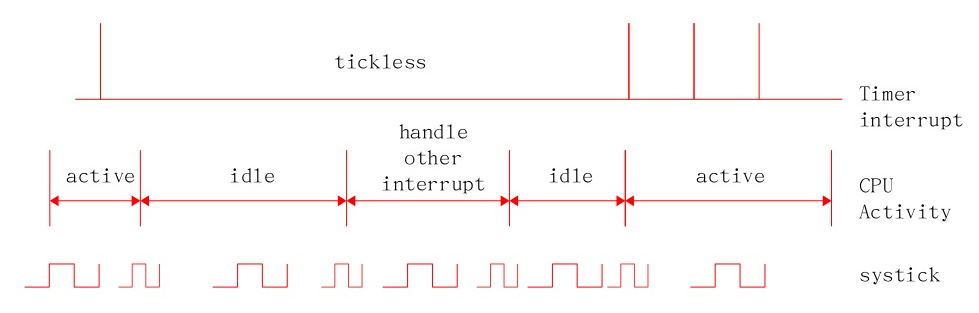
\includegraphics[width=\linewidth]{picture/tickless.png}
	\end{center}
	\caption{Tickless scheduling in f9-kernel}
\end{figure}


\subsection{bit-band and Ktable}
ARM Cortex-M provide an atomic access method call "Bit-banding", Bit-banding mechanisms is the device takes a region of memory (the Bit-band region) and maps each bit in that region to an entire word in a second memory region (the Bit-band Alias Region).\cite{schaenzle2013}

\begin{figure}[H]
\begin{center}
	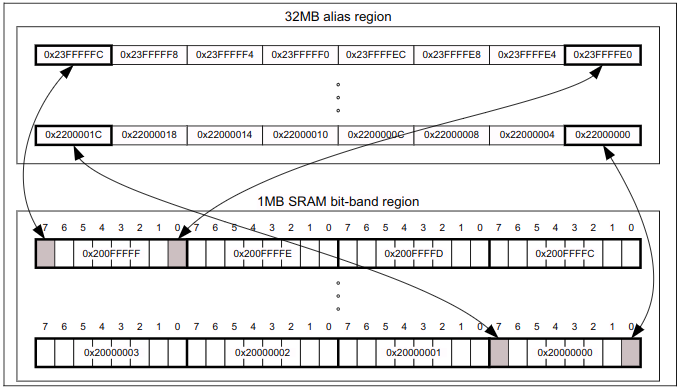
\includegraphics[width=\linewidth]{picture/bit-banding.png}
\end{center}
\caption{bit-banding in Cortex-M CPU\cite{st2016manual}}
\end{figure}

This techquine makes atomic access more friendly to developer since devloper won't using any assembly language and no need to take care about contex-switch or preemption problem.

f9-kernel using bit-band technique to create an fast atomic object management mechanism "Ktable", Ktable can create an structure that provide table size, number of chunk, and data. f9-kernel using Ktable to manage fpages table, address space table, and thread table.

\begin{itemize}
\footnotesize
\item \verb|void ktable_init(ktable_t *kt);|
\item \verb|int ktable_is_allocated(ktable_t *kt, int i);|
\item \verb|void *ktable_alloc_id(ktable_t *kt, int i);|
\item \verb|void *ktable_alloc(ktable_t *kt);|
\item \verb|void  ktable_free(ktable_t *kt, void *element);|
\item \verb|uint32_t ktable_getid(ktable_t *kt,void *ele);|
\end{itemize}


\begin{figure}[H]
	\begin{center}
		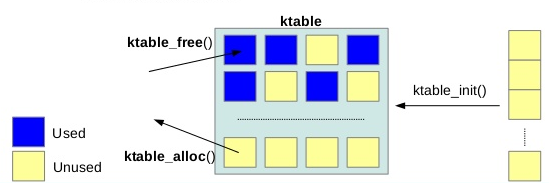
\includegraphics[width=\linewidth]{picture/ktable.png}
	\end{center}
	\caption{Manipulation in Ktable\cite{ncku2015}}
\end{figure}

\subsection{pthread mutex}
ARM Cortex-M provide an local exclusive monitor for exclusive accesses. This gave Cortex-M CPU have the atomic load / store ability for developers\cite{arm2012v7}. f9-kernel implement an POSIX compactiable library for user space, using atomic load / store technique, we are able to implement an user space mutex lock implement in pthread library.

Using thumb2 instruction, our approach in f9-kernel only need 24 bytes to implement the \texttt{pthread\_mutex\_trylock} function in pthread library.

\begin{lstlisting}[basicstyle=\small,frame=single]
44:	4603      	mov	r3, r0
46:	f04f 0101 	mov.w	r1, #1
4a:	461a      	mov	r2, r3
4c:	e852 0f00 	ldrex	r0, [r2]
50:	2800      	cmp	r0, #0
52:	bf04      	itt	eq
54:	e842 1000 	strexeq	r0, r1, [r2]
58:	4603      	moveq	r3, r0
5a:	4618      	mov	r0, r3
5c:	4770      	bx	lr
\end{lstlisting}

\section{Conclusion}
f9-kernel is the first microkernel that using MPU and create security memory management microkernel, rely on the fpage and address space infrastructure, f9-kernel can only waste a little memory space but provide thread to thread memory access control. Also f9-kernel have a fast IPC performance and tickless schedule for energy-saving, and provide f9-kernel a well in-kernel debugging toolchains like kdb and Kprobe.

The future work of f9-kernel can split into two catagories. One is to develop kernel itself, and another is to improve kernel dynamic tracing toolchains.

\bibliography{f9-report.bib}

\end{document}
